\chapter{Optimization with uncertain number of sold items}
\label{chap:unc_items}

\section{Contextual hypotesis}
\label{sec:unc_it_hyp}

In this case the e-commerce website doesn't register neither the units sold for each product nor the class parameters for the users.
Since this isn't a change that affects the enviroment directly, there will not be a separate mask to hide the \textit{units sold} to the learner, therefore the extra information will just be ignored by the learner.

We expect worse results overall since the learners are working with less data and therefore their prediction will have to factor in more uncertainty.

\section{Algorithm}
\label{sec:unc_it_alg}

The learner that we modelled for this specific scenario bares a lot of \textit{similarities} w.r.t. the learner used for the previous step as they both function following the same workflow.

However, in this case, the \texttt{learn} function is only allowed to gather information from the generic reward obtained for the day.

\begin{lstlisting}[style=Python]
def learn(self, _, reward: float, prediction: np.ndarray):
	for i, p in enumerate(prediction):
		prediction_index = np.where(self.budget_steps == p)[0][0]
		self.product_mabs[i].update(prediction_index, reward)
\end{lstlisting}

\clearpage % Aesthetic

\section{Results}
\label{sec:unc_it_res}

\vspace*{2em} % Aesthetic

\subsection{Single run reward and regret}

\vspace*{1em} % Aesthetic

Thompson Sampling and UCB

\begin{center}
	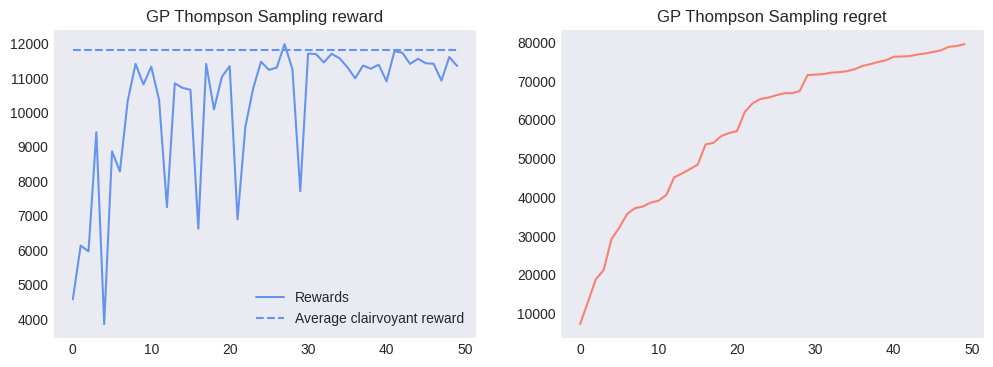
\includegraphics[scale=0.5]{img/Graphs/uncertain_alpha_unit/image1.png}
	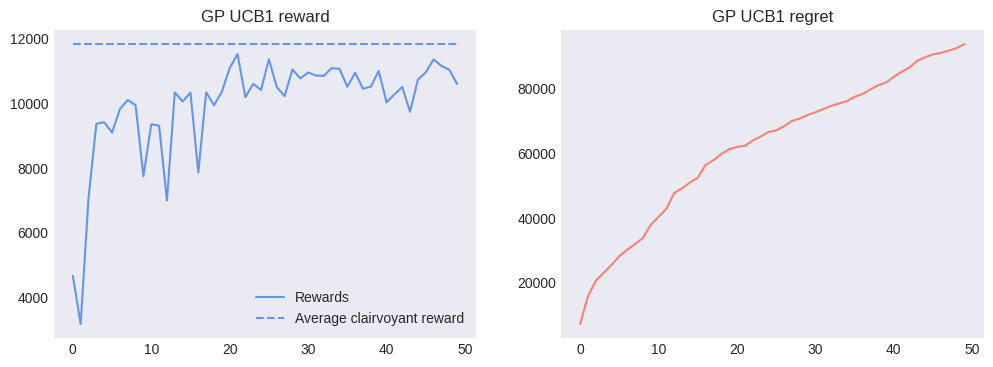
\includegraphics[scale=0.5]{img/Graphs/uncertain_alpha_unit/image2.png}
\end{center}

Regret comparison

\begin{center}
	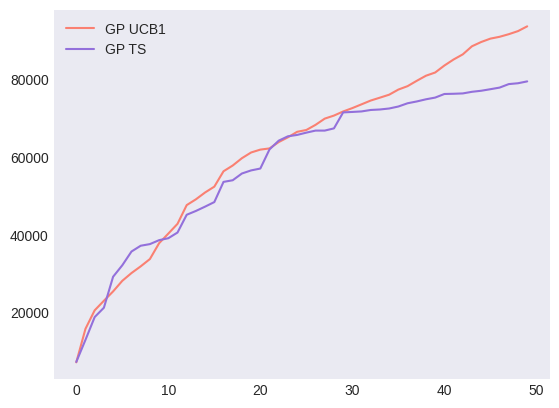
\includegraphics[scale=0.5]{img/Graphs/uncertain_alpha_unit/image3.png}
\end{center}

\clearpage % Aesthetic

\subsection{Average regret and reward}

\vspace*{1em} % Aesthetic

Thompson Sampling and UCB

\begin{center}
	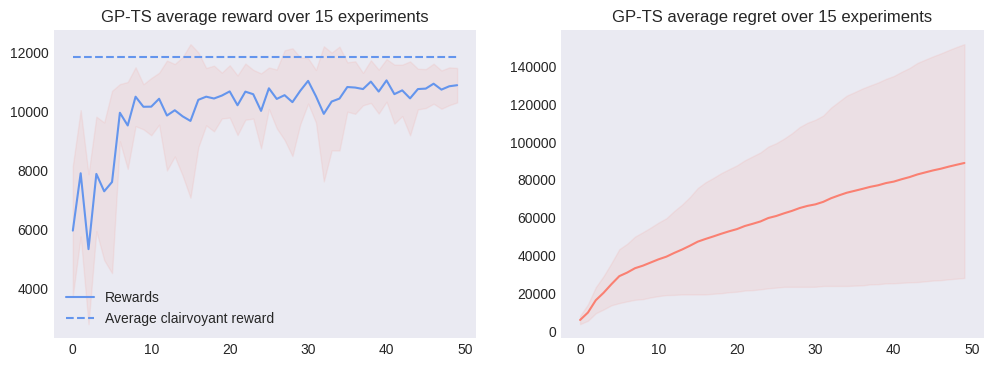
\includegraphics[scale=0.5]{img/Graphs/uncertain_alpha_unit/image4.png}
	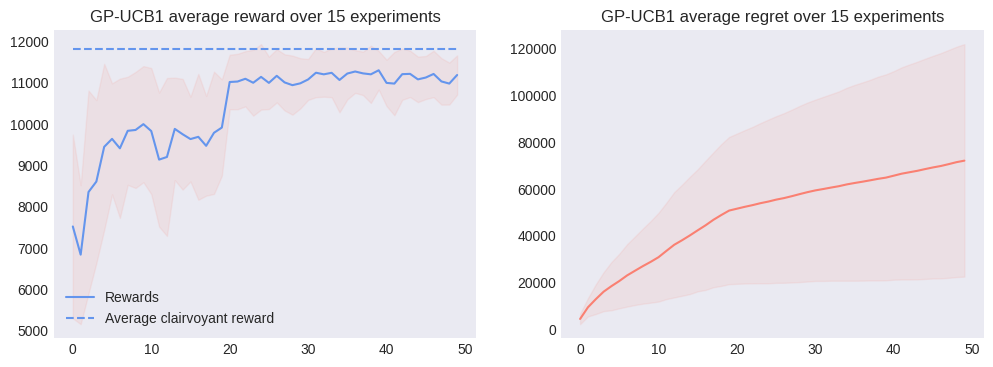
\includegraphics[scale=0.5]{img/Graphs/uncertain_alpha_unit/image5.png}
\end{center}

Average regret comparison

\begin{center}
	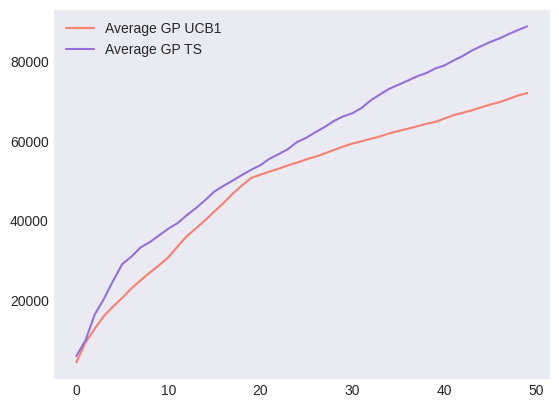
\includegraphics[scale=0.5]{img/Graphs/uncertain_alpha_unit/image6.png}
\end{center}

\clearpage % Aesthetic

\subsection{Conclusions}

In this scenario, results are clearly worse w.r.t. the previous step since the learners work with less information.

Both the TS and UCB approaches are not guaranteed to find the optimal arm as sometimes they seem to settle on a suboptimal solution, however we can see that the TS performance is much more unstable overall, this is also reflected in the average regret.

On average we can observe that UCB performs slightly better than TS probably due to a more unrealiable environment resulting in learners that are more "unsure" nullifying the advantage dictated by the randomness of the latter.

Average results over 15 runs at time horizon $T = 50$:

\begin{table}[h]
	\center
	\begin{tabular}{|c|cc|c|}
	\hline \hline
		\cellcolor{blue!25} & Reward 	& Regret	& Deviation \\
	\cline{2-4}
		\cellcolor{blue!25} & $\mu$		& $\mu$		& $\sigma$	\\
	\hline \hline
		GPTS 				& 10772.60	& 97205.53	& 904.08	\\
	\hline
		GPUCB				& 11029.20	& 72557.20	& 510.36	\\
	\hline \hline
	\end{tabular}
\end{table}
